\cotefile{81}
\scanpage{2}
\unsure{0|O}\quad \unsure{Cartes} sphériques en général
% archive sheet number: 1

\scanpage{3}
Carte sphérique \inserted{(\unsure{orientée})} avec repère (dans cat. \unsure{isotopique|isotopiques})

\[
\rotatebox{90}{$\simeq$}
\]
\unsure{morphisme} $\mathbb P^{1}_{\mathbb C}\overset{f}{\unsure{-|\longrightarrow}}\mathbb P^{1}_{\unsure{\mathrm C|\mathbb C}}$ ``\unsure{spécial}'' i.e
\[
 f(0)=0,\quad f(1)=1,\quad f(\infty)=\infty.\quad f\ \text{étale au dessus de }\mathbb P^{1}-\{0,1,\infty\}
\]
\[
\rotatebox{90}{$\simeq$}
\]
fonction rationnelle $f(z)$ telle que $f(0)=\deleted{\unsure{1}}0$, $f(1)=1$, $f(\infty)=\infty$ et telle que pour $z\in\mathbb C$ \deleted{telle que}\inserted{avec} $f(z)\deleted{\in}\notin\{0,\infty\}$ $f'(z)=0$, on ait $f(z)\deleted{\in}=1$ \deleted{\unsure{$\{0,1,\infty$}}\unsure{$\}$|,} \inserted{et de plus} $f''(z)\ne0$ (i.e. la ramification de $f$ en $z$ est $2$)\ldots.

\[
\rotatebox{90}{$\simeq$}
\]
couple $P,Q$ \inserted{$[f=P/Q\quad !\,]$} de polynômes $\in\mathbb C(z)$ premiers entre eux \inserted{(i.e. sans zéros communs)} tels que $P(0)=0$, (donc $Q(0)\ne0$) $P(1)=Q(1)$ (donc $\ne0$), $\deg Q<\deg P$ (ces conditions expriment \unsure{resp\textsuperscript{t}} $f(0)=0$, $f(1)=1$, $f(\infty)=\infty$)
% slanted
\margin{On pourrait aussi normaliser \unsure{au lieu de cel|au lieu de cela} par $Q(0)=1$, ou $P$ unitaire, ou $Q$ unitaire\ldots}
\unsure{normalisés} (par exemple) par $P(1)=Q(1)=1$, et tels que pour $z\in\mathbb C$ avec $[f(z)\deleted{\in}\notin\{0,\infty\}, f'(z)=0,\ \mathrm{i.e.}\,]$ \inserted{$P(z)\ne0$,} $Q(z)\ne0$,
\[
 \frac{P'(z)\deleted{\unsure{Q(z)}}}{P(z)}-\frac{Q'(z)}{Q(z)}=0,
\]
on ait $P(z)=Q(z)$, et de plus
\[
 \frac{P''(z)}{P(z)}-\frac{Q''(z)}{Q(z)}\ne0\qquad\text{i.e.}\quad P''(z)\ne Q''(z)\ldots
\]
[ NB on a
\[
\begin{aligned}
 Q(z)P'(z)-P(z)Q'(z)&=\deleted{Q(z)[P'(z)-P(z)]+P(z)(Q(z)-Q'(z))}\\
 &\phantom{=}\inserted{(Q(z)-P(z))P'(z)+P(z)(P'(z)-Q'(z))}
\end{aligned}
\]
donc si \inserted{pour $P(z);Q(z)\ne0$,} cette quantité est nulle, (i.e. $f'(z)=0$), alors $P(z)=Q(z)$ \deleted{\unsure{au|ou}} i.e $Q(z)-P(z)=0$ implique $P'(z)=Q'(z)$ et inversement si $P'(z)=Q'(z)$ on a $(Q(z)-P(z))P'(z)=0$ donc \uline{si} $P'(z)\ne0$, on a $P(z)=Q(z)$. Mais peut-on avoir $P'(z)=0$ (\unsure{d'où|donc} aussi $Q'(z)=0$) \inserted{avec $P'(z)=Q'(z)$}\unsure{$\}$|)} sans avoir $P(z)=Q(z)$ ?

\deleted{\unsure{Réfléchissons} \unsure{à} $Q(T)=$}

Prenons p.ex. $Q(\unsure{T})=1$, les \unsure{cond\textsuperscript{ns}} sur $P$ deviennent $P(0)=0$, $P(1)=1$, $\deg P\geq1$ \inserted{(conséquence des deux précédentes)}, donc $P(T)=\unsure{T}P_0(T)$ où on a $P_0(1)=1$, la question devient si on peut avoir \inserted{(pour $P(z)\ne0$)} $P'(z)=0$ sans avoir $P(z)=1$ certes oui p.ex. $\deleted{P(T)=T^2}$ si $P(T)=T(aT+b)=aT^2+bT$, $a+b=1$, on a
% margin note written sideways
\margin{\raggedright $P'(T)=2aT+b$ qui est nul \inserted{(supposons $a\ne0$)} pour $z=-\frac{b}{2a}$ \deleted{\unsure{sera}} $\ne\left\{\begin{smallmatrix}0\\-\frac{b}{a}\end{smallmatrix}\right.$ \deleted{\illegible{1}} les deux zéros de $P$ si $b\ne0$, et $P(-\frac{b}{2a})=-\frac{b}{2a}(-\frac b2+b)=-\frac{b^2}{4a}$ qui \deleted{\unsure{peut être}} est $\ne1$ \deleted{\unsure{en prenant}} si $b^2\ne-4a$\unsure{---}.}
% archive sheet number: 2

\scanpage{4}
% The two long diagonal cancellations traverse both columns. Local cancellations are nested.
\[
\deleted{\begin{aligned}
 f_{d-2}e_1&=-e_{d-2}f_1\qquad(=\unsure{\eta|\gamma}_{d-1}\unsure{\}|\,}= \eta)\\
 \delta(\eta)&=e_{d-2}
\end{aligned}}
\]
\[
\deleted{\boxed{\begin{gathered}
(1\leq i\leq d-2)\\
\left\{\begin{aligned}
e_i e_1&=0\qquad f_i f_1=\begin{cases}0&\text{si }i\text{ impair}\\f_{i+1}&\text{si }i\text{ pair}\end{cases}\\
f_i e_1&=e_{i+1}\\
e_i f_1&=\begin{cases}-e_{i+1}&\text{si }i\text{ impair}\\0&\text{si }i\text{ pair}\end{cases}
\end{aligned}\right.
\end{gathered}}}
\]
\[
\deleted{xf_1\unsure{=|\equiv}f_1x=0\quad\text{si }\deg x\text{ pair}\qquad
 \eta=e_{d-1}\quad \delta(e_{d-1})=e_{d-2}}
\]
\[
\deleted{\deleted{\unsure{xf_1}}}
\]
\[
\deleted{\begin{aligned}
 &(f_i+\lambda e_i)(f_1+\lambda e_1)\\
 &=\underset{\inserted{f_{i+1}}}{\deleted{f_i f_1}}+\lambda^2\deleted{e_i e_1}
 +\lambda\bigl(\underbrace{f_i e_1}_{\inserted{e_{i+1}}}+
 \underbrace{\deleted{e_i f_1}}_{\inserted{\deleted{\unsure{-}e_{i+1}}}}\bigr)
\end{aligned}}
\]
\[
\deleted{\begin{aligned}e_2&=f_1e_1\\e_3&=f_2e_1\end{aligned}}
\]
% margin note written upside down
\margin{\deleted{$\deleted{e_1 f_d}$}\quad
\deleted{$e_i e_1=0\qquad 1\leq i\leq d-2$}\quad
\deleted{$f_i f_1=$}}
\[
\deleted{\deleted{\delta(e_i e_j)=\unsure{0}}\qquad \delta(e_i e_j)=}
\]
\[
\deleted{\begin{gathered}
1\leq i\leq d-2\\
\left\{\begin{aligned}
e_i e_1&=0\\
f_i f_1&=\begin{cases}0&\text{si }i\text{ impair}\\ f_{i+1}&\text{si }i\text{ pair}\end{cases}\\
f_i e_1&=\eta_{i+1}=\alpha e_{i+1}+\beta f_{i+1}\\
e_i f_1&=\begin{cases}
-\deleted{\unsure{a|0}}\eta_{i+1}=-\alpha e_{i+1}-\beta f_{i+1}&i\text{ impair}\\
-\eta_{i+1}+e_{i+1}=(1-\alpha)e_{i+1}-\beta f_{i+1}&i\text{ pair}
\end{cases}
\end{aligned}\right.
\end{gathered}}
\]
\[
\deleted{\underline{f_1e_1\deleted{\unsure{f_1}}=-e_1f_1=\eta_2=\alpha e_2+\beta f_2}}
\]
\[
\deleted{\begin{gathered}
1\leq i\leq d-3\\
(e_i f_1)e_1=\deleted{\unsure{-e_i}}
\begin{cases}
-\eta_{i+1}e_1=-\beta f_{i+1}e_1=-\beta\eta_{i+2}&i\text{ imp}\\
-\eta_{i\unsure{-|+}1}\unsure{e|a}_1+\deleted{e_{i+1}e_1}=-\beta\eta_{i+2}&i\text{ pair}
\end{cases}\\
\rotatebox{90}{$=$}\\
e_i(f_1e_1)\deleted{=e_i\eta_2=e_i(\alpha e_2+\beta f_2)}\\
\rotatebox{90}{$=$}\\
-e_i(e_1 f_1)\\
\rotatebox{90}{$=$}\\
-(e_i e_1)f_1=0\qquad\text{donc}\quad
\tikz[baseline=(a.base)]\node[draw,circle,inner sep=1pt] (a) {$\beta=0$};\quad\alpha=\pm1
\end{gathered}}
\]
\[
\deleted{\text{donc}\quad\delta\eta=\pm e_{d-2}\qquad\unsure{Q\Phi S|QDS|QPS|QFS}}
\]
\[
\deleted{\begin{aligned}
\eta&=f_{d-2}e_1\\
\delta\eta&=\delta(f_{d-2})e_1=f_{d-3}e_1.
\end{aligned}}
\]
% archive sheet number: 3

\scanpage{5}
\uline{NB}\quad Si $\sigma$ est un \unsure{automorphisme} du corps des complexes, et si $f$ est ``spécial'', alors $f^\sigma$ est \unsure{égalmt|également} spécial -- donc $\operatorname{Aut}(\mathbb C)$ \unsure{opere|opère} sur l'ens des $f$ \unsure{spèciaux|spéciaux}. Mais il opère par l'intermédiaire de $\operatorname{Aut}(\unsure{\overline{\mathrm Q}|\overline{\mathbb Q}})$, car si $f=P/Q$ spécial, les coeff. de $P,Q$ sont des \uline{nbs algébriques}. Il \unsure{revient} au $=$ de dire que les zéros de $P,Q$ sont des nbs algébriques, i.e. le diviseur de $f$ est

\[
 \unsure{-|=}\hspace{5em}-
\]
% archive sheet number: 4

\scanpage{6}
\[
\begin{aligned}
(P/Q)'&=\frac{P'}{Q}-P\frac{Q'}{Q^2}=\frac{P'Q-Q'P}{Q^2}\\
(P/Q)''&=P''/Q\deleted{\unsure{+}}\unsure{-|+}2\frac{P'Q'}{Q^2}+\deleted{\unsure{2}}P\bigl(
\end{aligned}
\]
\[
\frac{P'}{\deleted{\unsure{Q}}P}-\frac{Q'}{Q}
\qquad (xy)^{\unsure{2|''}}=\unsure{x''|x^2}y+2x'y^{\unsure{\prime}}+xy^{\unsure{\prime\prime|\prime}}
\]
\[
\left(\frac{\deleted{\unsure{P'}}f}{g}\right)'=\frac{f'g-g'f}{g^2}
\]
\[
\frac{(P''Q+\deleted{P'Q'}-\deleted{P'Q'}\deleted{\unsure{+}}\unsure{-|+}Q''P)\deleted{Q}^{\,2}
 -(P'Q-Q'P)2\deleted{Q}Q'}{Q^{\unsure{3|4}}}
\]
\[
\frac{P''Q^2-Q''PQ-\unsure{2}P'QQ'+2PQ'^{\,2}}{Q^3}
\]
\[
2{\unsure{p|P}}^2Q^2\bigl(\unsure{-}\frac{Q'}{Q}+
\]

% Crossed writing in the opposite direction. Read after rotating the leaf by 180 degrees.
\[
\deleted{\det\begin{pmatrix}a\deleted{\unsure{d|b}}&c\\b&d\end{pmatrix}\unsure{-|=}ad-bc\quad\text{inversible}}
\]
\[
\deleted{\begin{aligned}
\delta(e_1 e_{d-2})&=-e_1\delta(e_{d-2})=-e_1e_{d-3}\deleted{\unsure{=e_d}}\\
&\rotatebox{90}{$=$}\\
\delta(a\unsure{\eta|\gamma})&=a\delta\eta=a\alpha e_{d-2}+a\beta f_{d-2}
\end{aligned}}
\]
\[
\deleted{\begin{aligned}
\delta(e_1 f_{d-2})&=-\deleted{\unsure{f}}e_1\cdot f_{d-3}\\
&\rotatebox{90}{$=$}\\
&b\alpha e_{d-2}+b\beta f_{d-2}
\end{aligned}}
\]
\[
\deleted{\begin{aligned}
\delta(f_1 e_{d-2})&=\delta(f_1)e_{d-2}-f_1\delta(e_{d-2})=e_{d-2}-f_1e_{d-3}\\
&\rotatebox{90}{$=$}\\
\delta(c\eta)&=c\delta\eta=c\alpha e_{d-2}+c\beta f_{d-2}
\end{aligned}}
\]
\deleted{etc}

\deleted{On en tire $e_1e_{d-3}$, $\deleted{\unsure{f}}e_1f_{d-3}$, $f_1e_{d-3}$, $f_1f_{d-3}$ comme \unsure{comb. lin} des $e_{d-1}$ et $f_{d-2}$, à coeff entiers \unsure{fonctions} de $\alpha,\beta$, $a,b,c,d$}

\[
\deleted{\begin{aligned}
\delta(e_1x_i)&=-e_1\delta(x_i)=-e_1\deleted{\unsure{\delta}}x_{i-1}\qquad 2\leq i\leq{}\\
&\rotatebox{90}{$=$}\\
\delta(\deleted{\unsure{S}}s e_{i+1}+t f_{i+1})&=s e_i+t f_i
\end{aligned}}
\]
% archive sheet number: 5

\scanpage{7}
\deleted{\illegible{1}} Soit $a\in\mathbb N^*,b\in\mathbb N^*,c\in\mathbb N^*,\ q\in\mathbb N^*$ \quad $q$ nombre premier $(q\ne1)$

On suppose que $a\mathrel{\underset{1}{\smile}}b$, $a\mathrel{\underset{1}{\smile}}c$, $b\mathrel{\underset{1}{\smile}}c$ (premiers entre eux deux à deux)
\inserted{et $a^q+b^q=c^q$}

On a $c>a$ et $c>b$ car $a\in\mathbb N^*$ et $b\in\mathbb N^*$

On pose $c=a+b'=b+a'$ avec $b'\in\mathbb N^*$ et $a'\in\mathbb N^*$
\[
\begin{aligned}
\text{alors}\qquad a^q+b^q=c^q&=(a+b')^q=\sum_{i=0}^{q}C_q^i\,a^i b'^{\,q-i}\qquad\text{(Newton)}\\
 &=b'^{\,q}+\sum_{i=1}^{q-1}C_q^i\,a^i b'^{\,q-i}+a^q\qquad(\text{car }q\geqslant2)
\end{aligned}
\]
\[
\text{donc}\qquad b^q=\sum_{i=1}^{q-1}C_q^i\,a^i b'^{\,q-i}+b'^{\,q}\tag*{(1)}
\]
la puissance de $b'$ n'étant jamais nulle on peut mettre $b'$ en facteur dans le second membre de (1), donc $b'\mid b^q$ ($b'$ divise $b^q$)

Soit $p$ un nombre premier \deleted{ou $p=1$} et tel que : $p\mid b'$ donc $p\mid b$. Soit $\alpha\in\mathbb N^*$ et $\alpha'\in\mathbb N^*$ tels que
\[
\begin{aligned}
 &p^{\alpha'}\mid b'\quad\text{et}\quad p^{\alpha'+1}\nmid b'\\
 \text{et}\quad &p^\alpha\mid b\quad\text{et}\quad p^{\alpha+1}\nmid b
\end{aligned}
\]
\margin{$\unsure{a|\alpha}$ \unsure{n'exist|n'existe} pas si on avait $p=1$}
On a $\alpha'\leqslant q\alpha$ car $b'\mid b^q$

\[
\begin{aligned}
(1)\ \Longrightarrow\quad&p^{q\alpha}\mid\sum_{i=1}^{q-1}C_q^i\,a^i b'^{\,q-i}+b'^{\,q}\\
\Longrightarrow\quad&p^{q\alpha}\mid b'\left(\sum_{i=1}^{q-1}C_q^i\,a^i b'^{\,q-i-1}+b'^{\,q-1}\right)\qquad(\text{car }q\geqslant2)
\end{aligned}
\]
posons $b'=p^{\alpha'}b''$ donc $b''\mathrel{\underset{1}{\smile}}p$ (propriété de $\alpha'$)
\[
\begin{aligned}
\Longrightarrow\quad&p^{q\alpha}\mid p^{\alpha'}b''\left(\sum_{i=1}^{q-1}C_q^i\,a^i b'^{\,q-i-1}+b'^{\,q-1}\right)\\
\Longrightarrow\quad&p^{q\alpha-\alpha'}\mid b''\left(\sum_{i=1}^{q-1}C_q^i\,a^i b'^{\,q-i-1}+b'^{\,q-1}\right)\quad\text{car }q\alpha\geqslant\alpha'\\
\Longrightarrow\quad&p^{q\alpha-\alpha'}\mid\sum_{i=1}^{q-1}C_q^i\,a^i b'^{\,q-i-1}+b'^{\,q-1}\quad\text{car }b''\mathrel{\underset{1}{\smile}}p
\end{aligned}
\]
% archive sheet number: 6

\scanpage{8}
Supposons que $q\alpha-\alpha'\ne0$ alors
\[
\begin{aligned}
(1)\ \Longrightarrow\quad &p\mid\sum_{i=1}^{q-1}C_q^i\,a^i b'^{\,q-i-1}+b'^{\,q-1}\\
\Longrightarrow\quad &p\mid q\,a^{q-1}\qquad\text{car }p\mid b'\ \text{et pour }i\ne q-1\quad q-i-1\deleted{\ne0}>0
\end{aligned}
\]
or $p\mid b'$ et $b'\mid b^q$ donc $b'\mathrel{\underset{1}{\smile}}a$ donc $p\mathrel{\underset{1}{\smile}}a$

\deleted{donc si $\unsure{p\ne1|p\ne q}$}
\[
(1)\ \Longrightarrow\quad p\mid q\qquad\text{donc }\deleted{p=1\ \text{ou }}p=q\quad(\text{si }q\alpha-\alpha'\ne0)
\]
Donc si $p\ne q$ \quad $p$ premier \inserted{ou $p=1$} et $p\mid b'$ alors $\alpha'=q\alpha$ \deleted{(on l'impose sans risque si $p=1$)}

Donc $\exists\,b_0\in\mathbb N^*$ et $\exists\,\gamma\in\mathbb N$ tel que $b'=q^\gamma b_0^q$ \margin{$q\nmid b_0$}

de plus $b_0\mid b$ et si $b=b_0 b''$ alors $b_0\mathrel{\underset{1}{\smile}}b''$ ?

De même $\exists\,a_0\in\mathbb N^*$ et $\exists\,\unsure{\zeta|\delta}\in\mathbb N$ tel que $a'=q^\zeta a_0^q$ avec $a_0\mid a$ et si $a=a_0a''$ alors $a_0\mathrel{\underset{1}{\smile}}a''$ ?

or $a\mathrel{\underset{1}{\smile}}b\Longrightarrow a_{\deleted{\unsure{0}}}'\mathrel{\underset{1}{\smile}}b'\Longrightarrow\zeta\times\gamma=0$ (et aussi $a_0\mathrel{\underset{1}{\smile}}b_0$)

Je suppose désormais que $\zeta=0$ donc $a'=a_0^q$

Donc \quad $c=b+a_0^q=a+q^\gamma b_0^q$
\margin{\begin{tikzpicture}[baseline=(n.base)]
\node[inner sep=2pt,text width=.85\marginparwidth] (n) {pour $q=2$ on a, $a_0=b_0=1$, $\gamma=1$, $b=4$, $a=3$, $c=5$};
\draw (n.north east) -- (n.north west) -- (n.south west) -- (n.south east);
\end{tikzpicture}}

\noindent\rule{\linewidth}{.35pt}\par
Je fais l'hypothése suivante \quad si $q$ premier et $1\leqslant i<q$ alors $q\mid C_q^i$
\par\noindent\rule{\linewidth}{.35pt}\par
alors Si $q\geqslant3$ et $q\alpha-\alpha'\geqslant2$ \deleted{\unsure{alors}} on a \inserted{$p=q,\ {\unsure{a|\alpha}}'=\gamma$}
\[
\begin{aligned}
(1)\ \Longrightarrow\quad &\deleted{\unsure{p^{2}|p}}q^2\mid q\,a^{q-1}\quad\deleted{\text{ou }p=1}\\
\Longrightarrow\quad&q\mid a^{q-1}\quad\deleted{\text{ou }p=1\Longrightarrow p=1}\ \inserted{\text{absurde car }q\nmid a}
\end{aligned}
\]
Donc $\gamma=0$ ou $\gamma={\deleted{q}}^{q\alpha-1}$ (sous réserve que l'hypothése est vraie)%
\margin{\begin{tikzpicture}[baseline=(n.base)]
\node[inner sep=0pt,text width=.85\marginparwidth] (n) {C'est peut-être interessant car ici $2$ est mis à part dans l'ensemble des nombres premiers};
\draw[->] (n.south east) -- ++(.16,0) |- (n.north east);
\end{tikzpicture}}
% archive sheet number: 7

\scanpage{10}
% crop-candidate: scan 10
\figure{%
\begin{tikzpicture}[x=.0056cm,y=-.0056cm,line cap=round,line join=round,line width=.57pt,
 every node/.style={font=\scriptsize,inner sep=1pt}]
% Upper row. Coordinates follow the scans, with y increasing toward the foot.
\draw (118,180) .. controls (96,175) and (65,165) .. (63,146) .. controls (60,125) and (74,98) .. (94,68) .. controls (114,54) and (139,53) .. (158,62) .. controls (185,75) and (200,102) .. (186,137) .. controls (174,168) and (147,184) .. (118,180) -- cycle;
\draw (80,83) .. controls (88,71) and (96,67) .. (99,65);
\draw (136,55) .. controls (127,87) and (124,146) .. (117,181);
\draw (318,164) .. controls (303,149) and (280,133) .. (288,110) .. controls (294,84) and (305,65) .. (324,65) .. controls (344,61) and (369,61) .. (385,78) .. controls (402,97) and (402,127) .. (387,146) .. controls (369,166) and (333,176) .. (318,164) -- cycle;
\draw (304,85)--(313,65) (292,83) .. controls (303,69) and (310,78) .. (316,72);
\draw (359,63) .. controls (347,100) and (337,144) .. (319,163);
\draw (386,75) .. controls (376,99) and (355,139) .. (359,165);
\draw (528,88) .. controls (548,68) and (579,74) .. (590,94) .. controls (606,122) and (591,152) .. (572,164) .. controls (549,174) and (523,169) .. (512,155) .. controls (495,128) and (504,101) .. (528,88) -- cycle;
\draw (505,107) .. controls (512,94) and (526,94) .. (530,85);
\draw (527,88) -- (544,125) -- (563,157);
\draw (512,158) -- (544,125) -- (579,82);
\fill (545,125) circle[radius=7.5];
\node at (568,39) {OK};
\draw (714,165) .. controls (692,138) and (707,102) .. (741,82) .. controls (763,71) and (805,69) .. (824,85) .. controls (845,101) and (838,140) .. (811,169) .. controls (783,190) and (740,190) .. (714,165) -- cycle;
\draw (750,82) .. controls (741,112) and (733,154) .. (716,171);
\draw (789,74) .. controls (771,116) and (760,159) .. (758,188);
\draw (821,83) .. controls (812,113) and (798,150) .. (809,171);
\draw (774,82) -- (788,74);
\draw (877,167) .. controls (874,143) and (884,111) .. (899,102) .. controls (914,94) and (943,93) .. (957,104) .. controls (971,119) and (978,145) .. (968,163) .. controls (951,183) and (921,193) .. (898,188) .. controls (882,184) and (875,177) .. (877,167) -- cycle;
\draw (899,101) .. controls (909,128) and (902,148) .. (877,166);
\draw (934,99) .. controls (946,117) and (947,134) .. (977,137);
\draw (898,186) .. controls (925,163) and (946,151) .. (968,162);
\draw (925,98)--(927,104) (934,98)--(940,106);
\draw (1007,168) .. controls (1007,137) and (1016,107) .. (1031,102) .. controls (1052,96) and (1065,106) .. (1066,128) .. controls (1065,157) and (1048,186) .. (1027,195) .. controls (1016,201) and (1009,184) .. (1007,168) -- cycle;
\draw (1015,118) -- (1031,130) -- (1063,132) (1008,170) -- (1032,129) -- (1057,103);
\draw (1015,194) .. controls (1031,167) and (1054,156) .. (1054,176);
\fill (1033,130) circle[radius=5.3];
\draw (1038,111)--(1055,103);
\draw (1089,170) .. controls (1094,140) and (1114,106) .. (1137,93) .. controls (1161,77) and (1199,88) .. (1222,101) .. controls (1246,124) and (1228,161) .. (1207,184) .. controls (1180,207) and (1144,214) .. (1121,202) .. controls (1102,193) and (1091,184) .. (1089,170) -- cycle;
\draw (1086,171) -- (1137,135) -- (1167,113) -- (1196,92);
\draw (1119,103) -- (1138,135) .. controls (1151,149) and (1170,178) .. (1184,195);
\draw (1156,86) .. controls (1161,103) and (1168,122) .. (1179,137) .. controls (1195,152) and (1201,165) .. (1217,172);
\draw[line width=3pt] (1138,135) -- (1167,113);
\node at (1153,55) {OK};
\draw (1306,198) .. controls (1298,178) and (1312,140) .. (1333,113) .. controls (1351,93) and (1383,82) .. (1400,89) .. controls (1420,98) and (1435,120) .. (1430,147) .. controls (1413,188) and (1379,216) .. (1344,216) .. controls (1326,214) and (1312,207) .. (1306,198) -- cycle;
\draw (1317,195)--(1397,89) (1328,115)--(1425,174) (1297,172) .. controls (1340,167) and (1385,161) .. (1436,139);
\fill (1338,166)--(1363,135)--(1394,153)--cycle;
\draw[line width=2pt] (1376,90) .. controls (1385,86) and (1397,86) .. (1404,94);
\node at (1376,52) {OK};
\draw (1490,75) .. controls (1477,75) and (1450,148) .. (1446,194) .. controls (1442,229) and (1454,246) .. (1486,240);
\node at (1495,165) {ou};
\draw (1554,177) .. controls (1552,150) and (1562,112) .. (1579,106) .. controls (1599,99) and (1624,111) .. (1633,135) .. controls (1642,163) and (1621,194) .. (1600,205) .. controls (1579,218) and (1555,209) .. (1554,177) -- cycle;
\draw (1566,129) .. controls (1578,149) and (1590,162) .. (1618,175);
\draw (1583,104) .. controls (1582,132) and (1587,174) .. (1597,205);
\draw (1568,206)--(1613,107);
\draw (1567,184) .. controls (1567,196) and (1567,206) .. (1571,209);
\draw[line width=1pt] (1592,178) .. controls (1591,196) and (1590,217) .. (1587,238);
\fill (1587,159) circle[radius=6.5];
\draw[opacity=.45] (1548,116) .. controls (1562,103) and (1574,101) .. (1584,102);
\draw (1632,96) .. controls (1647,66) and (1657,114) .. (1649,157) .. controls (1641,212) and (1624,259) .. (1606,273);
\draw (759,202) .. controls (780,226) and (799,220) .. (828,212) .. controls (843,208) and (846,205) .. (846,217) .. controls (872,197) and (918,220) .. (949,210) -- (944,207);
\draw[line width=.55pt] (746,274) .. controls (747,244) and (777,229) .. (821,226) .. controls (863,222) and (910,214) .. (923,230) .. controls (940,253) and (888,293) .. (840,300) .. controls (787,310) and (751,304) .. (746,282) -- cycle;
\draw[line width=.7pt] (949,271) .. controls (947,245) and (987,240) .. (1015,235) .. controls (1044,226) and (1072,217) .. (1068,255) .. controls (1064,295) and (1053,303) .. (1014,305) .. controls (969,310) and (951,299) .. (949,271) -- cycle;
\node[inner sep=0pt] at (121,235) {\begin{minipage}{75pt}
\diagram{\begin{tikzcd}[ampersand replacement=\&,column sep=4pt,row sep=0pt,cells={nodes={inner sep=0pt,outer sep=0pt}}]
\bullet
\end{tikzcd}}
\end{minipage}};
\node[inner sep=0pt] at (325,236) {\begin{minipage}{75pt}
\diagram{\begin{tikzcd}[ampersand replacement=\&,column sep=4.7pt,row sep=0pt,cells={nodes={inner sep=0pt,outer sep=0pt}}]
\bullet \& \bullet
\end{tikzcd}}
\end{minipage}};
\node[inner sep=0pt] at (533,233) {\begin{minipage}{75pt}
\diagram{\begin{tikzcd}[ampersand replacement=\&,column sep=13pt,row sep=0pt,cells={nodes={inner sep=0pt,outer sep=0pt}}]
\vphantom{\bullet}\arrow[r,dash,line width=.65pt,start anchor=center,end anchor=center,shorten <=1pt,shorten >=1pt] \& \vphantom{\bullet}
\end{tikzcd}}
\end{minipage}};
\node[inner sep=0pt] at (852,253) {\begin{minipage}{75pt}
\diagram{\begin{tikzcd}[ampersand replacement=\&,column sep=8pt,row sep=0pt,cells={nodes={inner sep=0pt,outer sep=0pt}}]
\bullet \& \bullet \& \bullet
\end{tikzcd}}
\end{minipage}};
\node[inner sep=0pt] at (1009,262) {\begin{minipage}{75pt}
\diagram{\begin{tikzcd}[ampersand replacement=\&,column sep=4pt,row sep=0pt,cells={nodes={inner sep=0pt,outer sep=0pt}}]
\vphantom{\bullet}\arrow[r,dash,line width=.65pt,start anchor=center,end anchor=center,shorten <=1pt,shorten >=1pt] \&[5.2pt] \vphantom{\bullet} \&[-2pt] \bullet
\end{tikzcd}}
\end{minipage}};
\node[inner sep=0pt] at (1152,251) {\begin{minipage}{75pt}
\diagram{\begin{tikzcd}[ampersand replacement=\&,column sep=8.3pt,row sep=0pt,cells={nodes={inner sep=0pt,outer sep=0pt}}]
\bullet\arrow[r,dash,line width=.65pt,start anchor=center,end anchor=center,shorten <=1pt,shorten >=1pt] \& \unsure{\bullet|\circ}\arrow[r,dash,line width=.65pt,start anchor=center,end anchor=center,shorten <=2.7pt,shorten >=1pt] \& \bullet
\end{tikzcd}}
\end{minipage}};
\node[inner sep=0pt] at (1326,262) {\begin{minipage}{75pt}
\diagram{\begin{tikzcd}[ampersand replacement=\&,column sep=1.2pt,row sep=2.0pt,cells={nodes={inner sep=0pt,outer sep=0pt}}]
{} \& \bullet\arrow[dl,dash,line width=.65pt]\arrow[dr,dash,line width=.65pt] \& {}\\
\bullet\arrow[rr,dash,line width=.65pt] \& {} \& \bullet
\end{tikzcd}}
\end{minipage}};
% Two small, detached ink traces near the upper edge.
\draw[opacity=.65,line width=.55pt] (1018,28)--(1025,29) (1037,27)--(1046,26);
% Middle row, left group.
\draw (116,390) .. controls (129,357) and (164,337) .. (200,327) .. controls (226,322) and (254,320) .. (272,326) .. controls (307,338) and (328,377) .. (326,413) .. controls (324,455) and (301,485) .. (265,500) .. controls (239,512) and (207,515) .. (184,510) .. controls (147,506) and (125,480) .. (116,455) .. controls (111,433) and (112,411) .. (116,390) -- cycle;
\draw (122,399) .. controls (122,392) and (126,388) .. (131,388);
\draw (154,353) .. controls (158,379) and (146,454) .. (128,472);
\draw (205,327) .. controls (203,354) and (205,404) .. (201,431) .. controls (197,465) and (193,491) .. (191,513);
\draw (270,324) .. controls (258,366) and (252,404) .. (253,433) .. controls (252,456) and (256,486) .. (263,501);
\draw (311,367) .. controls (296,393) and (290,441) .. (305,475);
\draw[opacity=.2] (192,503)--(195,556);
\draw (400,505) .. controls (378,492) and (374,467) .. (377,444) .. controls (382,413) and (403,377) .. (420,364) .. controls (441,342) and (462,334) .. (482,340) .. controls (514,337) and (544,366) .. (542,403) .. controls (543,444) and (508,491) .. (484,503) .. controls (462,516) and (428,521) .. (400,505) -- cycle;
\draw (419,365) .. controls (426,377) and (409,469) .. (400,503);
\draw (482,343) .. controls (461,390) and (451,446) .. (449,510);
\draw (517,356) .. controls (502,397) and (484,451) .. (481,501);
\draw[line width=1.6pt] (406,503) .. controls (423,481) and (428,504) .. (433,517);
\draw (433,512)--(434,519) (448,491)--(447,513) (456,346)--(482,340);
\draw (568,459) .. controls (563,432) and (570,399) .. (581,379) .. controls (594,358) and (612,345) .. (640,352) .. controls (665,358) and (685,385) .. (687,411) .. controls (693,446) and (680,490) .. (647,519) .. controls (636,523) and (624,523) .. (609,524) .. controls (590,517) and (571,499) .. (568,480) -- cycle;
\draw (598,359) .. controls (613,387) and (599,433) .. (567,459);
\draw (645,353) .. controls (653,386) and (676,407) .. (693,410);
\draw (570,480) .. controls (590,487) and (605,503) .. (610,524);
\draw[line width=1pt] (644,519) .. controls (647,504) and (665,473) .. (682,462);
\draw[line width=1.8pt] (684,395) .. controls (697,432) and (683,488) .. (651,516);
\draw (178,557) .. controls (177,574) and (221,577) .. (266,570) .. controls (311,564) and (361,554) .. (376,584) .. controls (378,560) and (416,560) .. (439,563) .. controls (497,573) and (539,558) .. (631,549);
\fill (733,427) circle[radius=2]; \fill (713,443) circle[radius=1.1];
% Middle row, right group.
\draw (778,444) .. controls (795,393) and (841,368) .. (889,367) .. controls (926,365) and (959,385) .. (977,414) .. controls (1001,449) and (966,489) .. (944,514) .. controls (923,544) and (901,563) .. (874,562) .. controls (842,564) and (800,553) .. (774,526) .. controls (774,509) and (771,472) .. (778,444) -- cycle;
\draw (772,446) .. controls (815,439) and (889,422) .. (947,388);
\draw (790,536) -- (854,425) -- (891,367);
\draw (778,464) .. controls (801,466) and (800,495) .. (777,509);
\draw (909,368) .. controls (910,392) and (925,388) .. (937,375);
\draw (774,517) .. controls (783,516) and (781,535) .. (791,536);
\fill (855,425) circle[radius=7.6];
\draw (990,500) .. controls (989,465) and (1002,432) .. (1026,409) .. controls (1047,386) and (1072,381) .. (1088,394) .. controls (1114,409) and (1110,444) .. (1104,473) .. controls (1098,508) and (1073,550) .. (1052,568) .. controls (1023,582) and (1009,571) .. (1000,548) .. controls (994,529) and (990,511) .. (990,500) -- cycle;
\draw (1021,412) .. controls (1043,438) and (1062,481) .. (1078,517);
\draw (998,534) .. controls (1023,505) and (1065,431) .. (1091,399);
\draw (998,456) .. controls (1018,463) and (1009,490) .. (991,501);
\draw (1015,570) .. controls (1034,544) and (1052,547) .. (1057,562);
\fill (1053,458) ellipse[x radius=6.8,y radius=9];
\draw (1133,512) .. controls (1136,476) and (1157,427) .. (1183,402) .. controls (1209,376) and (1248,380) .. (1268,395) .. controls (1296,420) and (1293,459) .. (1285,493) .. controls (1274,530) and (1241,562) .. (1208,571) .. controls (1171,582) and (1146,555) .. (1137,534) .. controls (1133,523) and (1132,516) .. (1133,512) -- cycle;
\draw (1172,411) -- (1207,472) .. controls (1222,498) and (1233,526) .. (1243,551);
\draw (1144,552) .. controls (1161,534) and (1218,450) .. (1266,395);
\draw (1155,453) .. controls (1175,478) and (1159,506) .. (1133,523);
\draw (1159,444) .. controls (1166,453) and (1181,440) .. (1171,428);
\fill (1207,472) circle[radius=7.3];
\draw (1285,514) .. controls (1291,476) and (1311,437) .. (1337,415) .. controls (1356,400) and (1381,409) .. (1391,423) .. controls (1417,463) and (1404,507) .. (1384,535) .. controls (1369,559) and (1349,583) .. (1327,588) .. controls (1306,591) and (1288,575) .. (1284,550) .. controls (1281,536) and (1282,525) .. (1285,514) -- cycle;
\draw (1315,444) -- (1342,491) -- (1368,559);
\draw (1290,564) .. controls (1307,552) and (1355,466) .. (1388,423);
\draw (1299,575) .. controls (1317,554) and (1335,524) .. (1347,555) -- (1353,570);
\draw (1312,585) .. controls (1328,561) and (1340,561) .. (1340,582);
\fill (1343,492) circle[radius=6.6];
\fill (1307,505) .. controls (1310,497) and (1314,496) .. (1318,483) .. controls (1324,477) and (1329,500) .. (1324,509) .. controls (1317,520) and (1305,515) .. (1307,505) -- cycle;
\draw (1328,433) .. controls (1330,406) and (1335,357) .. (1341,329);
\draw[line width=1.8pt] (1327,436) .. controls (1335,425) and (1340,416) .. (1349,418);
\draw (793,583) .. controls (822,621) and (923,616) .. (981,613) .. controls (1025,612) and (1060,623) .. (1079,622) .. controls (1090,628) and (1095,637) .. (1102,649) .. controls (1114,632) and (1127,626) .. (1138,621) .. controls (1220,627) and (1280,619) .. (1348,616) .. controls (1354,610) and (1360,601) .. (1364,592);
\draw (1004,605) .. controls (1015,626) and (1050,615) .. (1069,622) (1167,622) -- (1204,630);
\node[font=\bfseries\small] at (539,658) {?};
\node[inner sep=0pt] at (373,646) {\begin{minipage}{85pt}
\diagram{\begin{tikzcd}[ampersand replacement=\&,column sep=7pt,row sep=0pt,cells={nodes={inner sep=0pt,outer sep=0pt}}]
\bullet \& \bullet \& \bullet \& \bullet
\end{tikzcd}}
\end{minipage}};
\node[inner sep=0pt] at (848,648) {\begin{minipage}{85pt}
\diagram{\begin{tikzcd}[ampersand replacement=\&,column sep=11.1pt,row sep=0pt,cells={nodes={inner sep=0pt,outer sep=0pt}}]
\vphantom{\bullet}\arrow[r,dash,line width=.65pt,start anchor=center,end anchor=center,shorten <=1pt,shorten >=1pt] \& \vphantom{\bullet} \& \bullet \& \bullet
\end{tikzcd}}
\end{minipage}};
% Lower row.
\draw[opacity=.22,line width=.4pt] (1518,375) .. controls (1540,374) and (1561,405) .. (1524,401);
\fill[opacity=.75] (1566,580) circle[radius=1.25]; \fill[opacity=.65] (1561,587) circle[radius=1];
\node at (201,691) {OK};
\draw (123,811) .. controls (135,770) and (168,740) .. (208,726) .. controls (239,716) and (275,725) .. (304,749) .. controls (339,775) and (354,809) .. (350,840) .. controls (347,879) and (314,935) .. (279,960) .. controls (257,972) and (226,969) .. (198,968) .. controls (162,965) and (130,943) .. (121,913) .. controls (114,887) and (118,844) .. (123,811) -- cycle;
\draw (124,893) .. controls (149,863) and (184,800) .. (219,718);
\draw (125,813) -- (194,773) .. controls (223,757) and (257,743) .. (274,727);
\draw (198,968) -- (298,838) -- (340,790);
\draw (277,965) .. controls (283,927) and (291,876) .. (298,839) .. controls (303,812) and (307,781) .. (310,754);
\fill (194,773) circle[radius=7.5]; \fill (299,838) circle[radius=7];
\draw[opacity=.4] (276,827)--(293,828);
\node[inner sep=0pt,outer sep=0pt,anchor=center] at (548,820) {\deleted{\hbox{\begin{tikzpicture}[x=.0056cm,y=-.0056cm,line cap=round,line join=round,line width=.57pt]
\path[use as bounding box] (450,714) rectangle (646,926);
\draw (460,830) .. controls (473,785) and (509,749) .. (541,731) .. controls (566,724) and (595,741) .. (613,754) .. controls (645,781) and (638,817) .. (626,842) .. controls (605,883) and (571,914) .. (538,917) .. controls (508,924) and (480,912) .. (462,889) .. controls (452,874) and (454,848) .. (460,830) -- cycle;
\draw (474,789) -- (612,754) (461,891) -- (547,729) (556,729) .. controls (578,778) and (605,805) .. (628,838);
% Repeated diagonal cancellation strokes in this disk.
\draw (535,717) .. controls (526,729) and (457,833) .. (461,835) .. controls (470,838) and (538,725) .. (537,729) .. controls (515,764) and (465,860) .. (470,865) .. controls (476,870) and (554,747) .. (565,747) .. controls (549,777) and (493,861) .. (493,865) .. controls (504,870) and (569,753) .. (585,751) .. controls (557,783) and (513,860) .. (518,866) .. controls (526,877) and (601,791) .. (614,798) .. controls (618,801) and (589,843) .. (563,892) .. controls (554,907) and (560,914) .. (572,923);
\end{tikzpicture}}}};
\draw (666,836) .. controls (669,808) and (686,789) .. (706,785) .. controls (725,782) and (746,786) .. (755,803) .. controls (773,824) and (771,857) .. (758,880) .. controls (746,903) and (728,917) .. (706,910) .. controls (683,903) and (660,871) .. (666,836) -- cycle;
\draw (707,786) -- (694,902) (747,789) .. controls (739,827) and (735,869) .. (729,906);
\draw (666,840)--(767,844);
\draw[line width=3.4pt] (699,838)--(737,842);
\draw (718,786) .. controls (715,814) and (733,813) .. (737,789);
\draw (797,850) .. controls (804,822) and (821,801) .. (839,798) .. controls (864,797) and (876,815) .. (881,839) .. controls (890,866) and (876,895) .. (860,910) .. controls (841,926) and (822,917) .. (809,905) .. controls (796,890) and (792,870) .. (797,850) -- cycle;
\draw (827,805) .. controls (823,843) and (819,878) .. (816,915);
\draw (862,805) .. controls (858,842) and (854,879) .. (852,914);
\draw (799,861)--(890,859); \draw[line width=2.8pt] (820,857)--(853,857);
\draw (874,818) .. controls (868,841) and (868,848) .. (885,850);
\draw (543,948) .. controls (573,976) and (607,963) .. (665,954) .. controls (706,949) and (731,945) .. (741,967) .. controls (744,947) and (789,945) .. (826,944) .. controls (864,943) and (881,941) .. (899,937) -- (898,931);
\node at (1156,724) {OK};
\draw (1004,849) .. controls (1005,815) and (1033,783) .. (1069,769) .. controls (1101,757) and (1134,762) .. (1150,787) .. controls (1172,815) and (1183,855) .. (1165,903) .. controls (1149,943) and (1125,964) .. (1109,969) .. controls (1072,976) and (1040,970) .. (1024,945) .. controls (1004,913) and (997,879) .. (1004,849) -- cycle;
\draw[opacity=.65] (1006,850) .. controls (1002,859) and (1003,869) .. (1009,874);
\draw (1012,924) .. controls (1029,875) and (1050,817) .. (1070,770);
\draw (1011,808) .. controls (1055,804) and (1125,796) .. (1156,788);
\draw (1101,764) .. controls (1110,780) and (1116,791) .. (1120,798) -- (1174,881);
\draw (1109,967) .. controls (1127,926) and (1154,855) .. (1172,823);
\draw[line width=2.7pt] (1056,802)--(1119,794);
\draw[line width=3.7pt] (1118,795)--(1158,853);
% Two faint, angular lines at the foot, crossing the last graph and continuing at the right.
\draw[opacity=.55] (1010,975) .. controls (1027,995) and (1035,1030) .. (1044,1050) .. controls (1053,1074) and (1061,1090) .. (1075,1089);
\draw[line width=1.5pt] (1041,1036) .. controls (1052,1070) and (1060,1090) .. (1074,1088);
\draw[opacity=.16] (1073,1088) .. controls (1108,1087) and (1162,1076) .. (1214,1064) -- (1288,985);
\draw[opacity=.5] (1215,1073)--(1237,1044) (1246,1033)--(1261,1014) (1278,996)--(1289,982);
\draw[opacity=.22] (1345,934) .. controls (1353,954) and (1350,994) .. (1358,1009) -- (1372,1014);
\draw[line width=1.9pt] (1373,1014) .. controls (1390,1025) and (1430,1037) .. (1458,1048) -- (1484,1054) -- (1500,1036);
\draw[opacity=.5] (1487,1054)--(1581,957);
\draw[opacity=.23] (1568,905) .. controls (1572,924) and (1571,943) .. (1581,957);
\node[inner sep=0pt] at (222,1035) {\begin{minipage}{94pt}
\diagram{\begin{tikzcd}[ampersand replacement=\&,column sep=5.2pt,row sep=0pt,cells={nodes={inner sep=0pt,outer sep=0pt}}]
\unsure{\bullet|\circ}\arrow[r,dash,line width=.65pt,start anchor=center,end anchor=center,shorten <=1pt,shorten >=1pt] \& \circ \& \hspace{3.3pt} \& \bullet\arrow[r,dash,line width=.65pt,start anchor=center,end anchor=center,shorten <=1pt,shorten >=1pt] \& \bullet
\end{tikzcd}}
\end{minipage}};
\node[inner sep=0pt] at (563,1026) {\begin{minipage}{94pt}
\diagram{\begin{tikzcd}[ampersand replacement=\&,column sep=7pt,row sep=0pt,cells={nodes={inner sep=0pt,outer sep=0pt}}]
\bullet\arrow[r,dash,line width=.65pt,start anchor=center,end anchor=center,shorten <=1pt,shorten >=1pt] \& \bullet\arrow[r,dash,line width=.65pt,start anchor=center,end anchor=center,shorten <=2.7pt,shorten >=1pt] \& \bullet \& \bullet
\end{tikzcd}}
\end{minipage}};
\node[inner sep=0pt] at (1075,1032) {\begin{minipage}{94pt}
\diagram{\begin{tikzcd}[ampersand replacement=\&,column sep=9pt,row sep=0pt,cells={nodes={inner sep=0pt,outer sep=0pt}}]
\bullet\arrow[r,dash,line width=.65pt,start anchor=center,end anchor=center,shorten <=1pt,shorten >=1pt] \& \bullet\arrow[r,dash,line width=.65pt,start anchor=center,end anchor=center,shorten <=1pt,shorten >=1pt] \& \bullet\arrow[r,dash,line width=.65pt,start anchor=center,end anchor=center,shorten <=1pt,shorten >=1pt] \& \bullet
\end{tikzcd}}
\end{minipage}};
\end{tikzpicture}}
% archive sheet number: 9

